\documentclass{article}
\usepackage{lgrind}
\usepackage{fullpage}
\usepackage{graphicx}

\author{Bo Shi}
\title{6.111 Lab Report 2 \\ Traffic Light Controller}
\date{October 13, 2004}


\begin{document}

\maketitle

\begin{abstract}
This report details the design and implementation of the traffic light controller.
\end{abstract}

\newpage
% \pagenumbering{roman}
% \setcounter{page}{1}
\tableofcontents

\newpage
\listoffigures 
\listoftables 

\newpage
% \pagenumbering{arabic}
% \setcounter{page}{1}
\section{Design Overview}
	blah abalha aga og

	\subsection{Setup}
		The four inputs to the controller were push buttons.  The
		output was a 7-bit value ordered as the figure shows.
		The FPGA used was an Altera Flex 10K10 clocked with a 1.8432 Mhz
		crystal oscillator.
	

	\subsection{Module Overview}
		\subsubsection{Synchronizer}
			This module synchronizes asynchronous input from the
			push buttons.  The RESET, WALK\_REQUEST, and REPROGRAM
			signals are converted to pulses while the SENSOR input
			is only synchronized.

		\subsubsection{Walk Register}
			The walk register is a very simple module containing a
			register and some additional control logic.  A walk
			request pulse will set the value in the register high
			and the signal will remain high until after the request
			as been granted.

		\subsubsection{Finite State Machine (FSM)}
			The specifications for operation are discussed in
			subsequent sections.

		\subsubsection{Time Parameters}
			This module determines the duration of a given state
			as requested by the FSM module.  Three different
			durations are available (see Figure 

		\subsubsection{Timer}
			The timer module signals the FSM upon the end of the
			time duration specified by the time parameters module.

		\subsubsection{Divider}
			The divider sends out a pulse every second.  The c

\section{Module Implementation}
	\subsection{Walk Register}
		The walk register module has an internal bit that is set to
		high when a walk signal has been requested.  When the FSM exits
		the \texttt{walk} state, a \texttt{wr\_reset} pulse is sent and
		gives the register a value of zero.

	\subsection{Timer}
		The timer keeps an internal 4-bit counter.  When it recieves a
		pulse from the Divider module, the counter decrements.  When
		the counter's value is one, it sends out an {\texttt{expired}}
		pulse to the FSM.  Upon reception of a {\texttt{start\_timer}}
		pulse, the Timer will load a new counter value from the Time
		Parameter module and begin counting down.

	\subsection{Time Parameters}
		The specification states that the time parameters should be
		programmable.  On the \texttt{prog\_sync} pulse, the module will
		read the 4--bit time value (the input ``Time Value'' in
		Figure~\ref{fig:block} and program the interval selected by the 2--bit
		select signal (the input ``Time Parameter Selector'').
		It is possible that an error might cause a value of zero might be
		programmed as one of the time parameters.  Since the \texttt{expired}
		signal is only sent when the timer counter has value 1, a programmed
		value of zero will simply cause the time parameter to become 16 seconds
		long.

	\subsection{Divider}
		The divider maintains a N-bit counter capable of holding a
		value larger and or equal to the clock frequency.  The clock
		used for the traffic light controller is a 1.8432 Mhz crystal
		oscillator.  Consequently, each time the Divider counter
		reached 1,843,200, the counter was reset and the {\texttt{
		onehzenable}} pulse was sent to the Timer.

	\begin{figure}
	\centering
	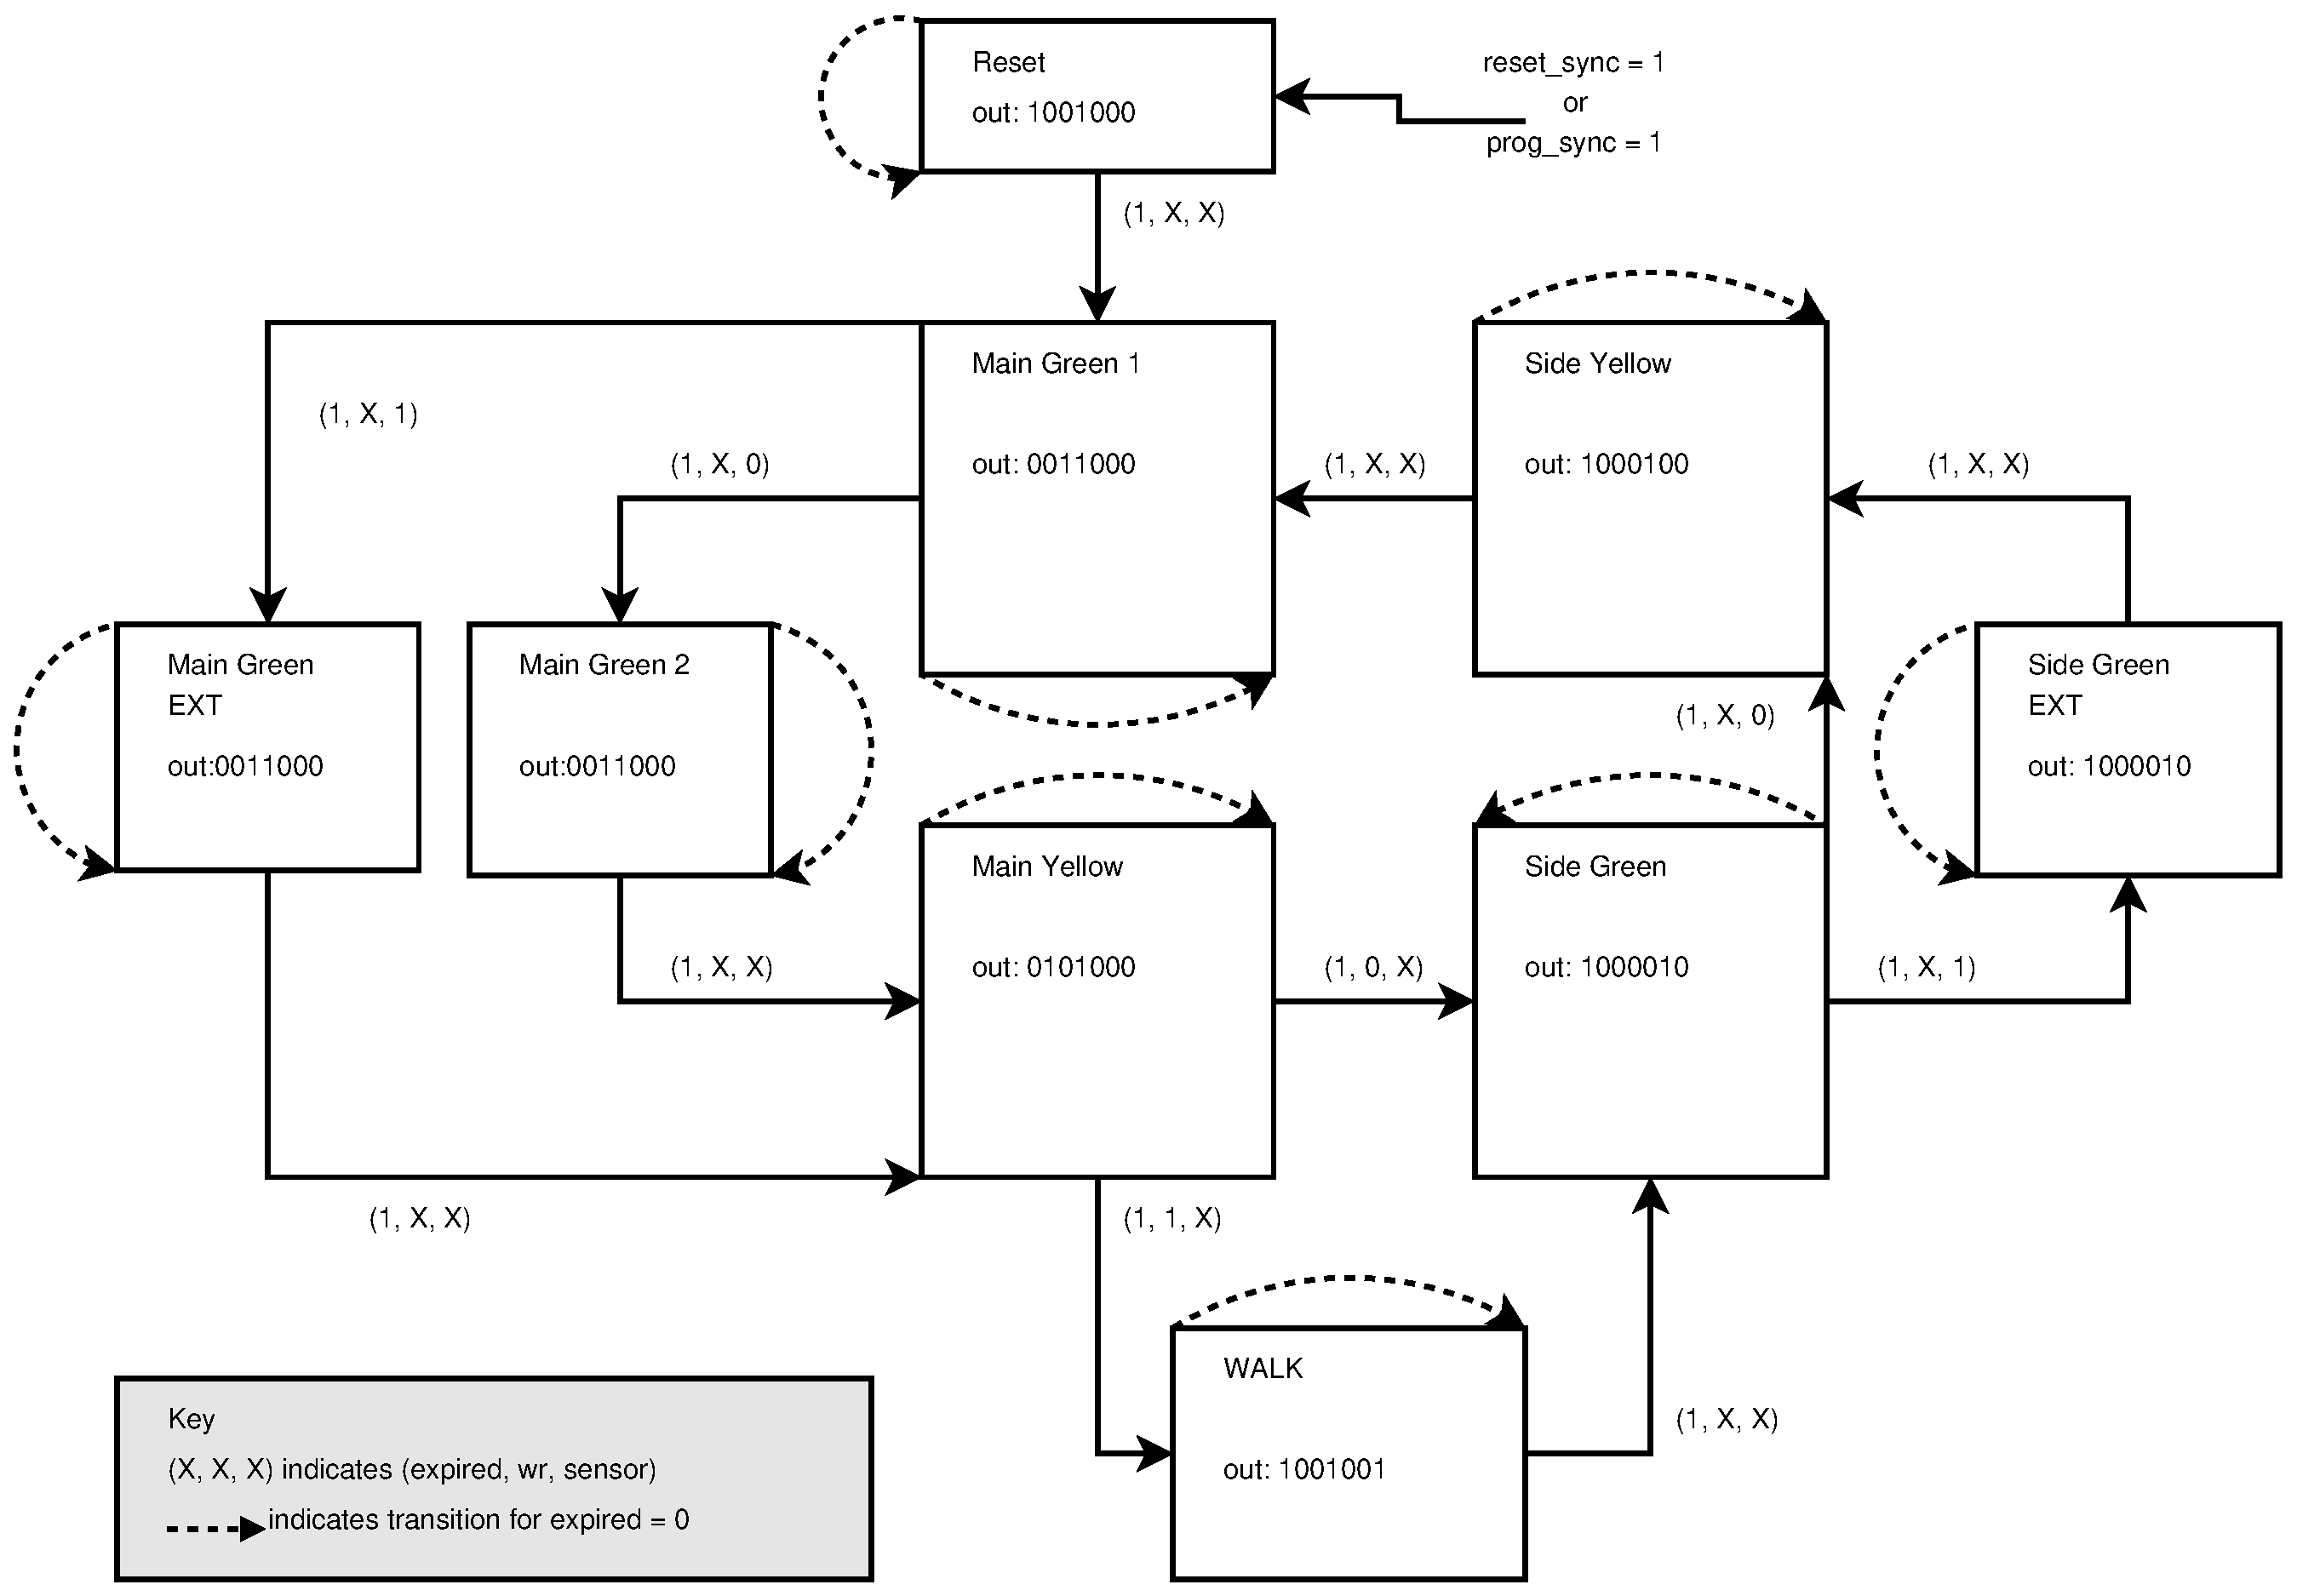
\includegraphics{fsm.ps}
	\caption{Finite State Machine for the Traffic Light Controller}
	\label{fig:fsm}
	\end{figure}

	\subsection{Finite State Machine}
		Figure~\ref{fig:fsm} shows the finite state machine controlling
		the lights.

		When RESET is asserted, the FSM enters the \texttt{S\_RESET}
		state\footnote{The original design used \texttt{S\_main\_green} as both
		the initial state and the reset state.  This was changed because the
		behavior of the design is not particularly safe.  If the reset were to
		be asserted during actual operation, it would be best to have a period
		of all red lights so that actual traffic does not get adversely
		confused.}.  The \texttt{S\_RESET} state lasts for 3 seconds and then
		the controller starts normal operation.  Normal operation 
	
	\begin{table}
	\centering
		\begin{tabular}{|c|c|c|c|c|}
		\hline
		Interval Name & Symbol & Parameter Number & Default $\Delta$t (s) & Time Value \\ \hline
		Base & $t_{base}$ & \texttt{00} & 6 & \texttt{0110} \\ \hline
		Extended & $t_{ext}$ & \texttt{01} & 3 & \texttt{0011} \\ \hline
		Yellow & $t_{yel}$ & \texttt{10} & 2 & \texttt{0010} \\ \hline
		\end{tabular}
	\caption{Default Timing Parameters}
	\label{tbl:timeparam}
	\end{table}


\section{Debugging}
	...Was a pain in the ass.

	The timer originally sent the \texttt{expired} signal when it's counter
	reached zero.  This caused two problems observed in simulation.  First,
	the intervals all lasted 1 second longer than necessary.  Second, attempting
	to program 0 into the time parameters would cause the FSM to lock into whichever
	parameter was zero.  Making the pulse fire when the timer counter reached
	the value 1 would solve both these problems.

	The most complex interaction was between the FSM, Time Parameter, and
	Timer module.  The MUX was synchronized -- this caused a problem where
	the initial test results reported that there was an off-by-one error
	for the intervals.  The Timer was recieving 'value' signals one clock
	cycle too early.

\section{Conclusions}

\newpage
\section{Appendix: Source Code Listing}
	\subsection{Step to Pulse Module}
		\begin{lgrind}
		\input exsync.v.latex
		\end{lgrind}

	\subsection{Synchronizer}
		\begin{lgrind}
		\input synchronizer.v.latex
		\end{lgrind}

	\subsection{Walk Register}
		\begin{lgrind}
		\input walkregister.v.latex
		\end{lgrind}

	\subsection{Finite State Machine}
		\begin{lgrind}
		\input fsm.v.latex
		\end{lgrind}

	\subsection{Time Parameters}
		\begin{lgrind}
		\input timeparams.v.latex
		\end{lgrind}

	\subsection{Timer}
		\begin{lgrind}
		\input timer.v.latex
		\end{lgrind}

	\subsection{Divider}
		\begin{lgrind}
		\input divider.v.latex
		\end{lgrind}

	\subsection{Top Level Module}
		\begin{lgrind}
		\input controller.v.latex
		\end{lgrind}

\end{document}
